\documentclass[12pt]{article}

\usepackage{mla13}

% ========== Note to users =========
% Remove these two packages after 
% you remove the example text.
\usepackage{graphicx}
\usepackage{lipsum}
\usepackage{amsfonts}
\usepackage{booktabs}
\usepackage{tikz}
\usepackage{amsmath}
\usepackage{amsthm}
\usepackage{array}
\usetikzlibrary{positioning}

\usepackage{listings}
\usepackage{color}

\definecolor{dkgreen}{rgb}{0,0.6,0}
\definecolor{gray}{rgb}{0.5,0.5,0.5}
\definecolor{mauve}{rgb}{0.58,0,0.82}

\lstset{frame=tb,
  language=Python,
  aboveskip=3mm,
  belowskip=3mm,
  showstringspaces=false,
  columns=flexible,
  basicstyle={\small\ttfamily},
  numbers=none,
  numberstyle=\tiny\color{gray},
  keywordstyle=\color{blue},
  commentstyle=\color{dkgreen},
  stringstyle=\color{mauve},
  breaklines=true,
  breakatwhitespace=true,
  tabsize=3
}

\newtheorem{theorem}{Theorem}
\theoremstyle{definition}
\newtheorem{definition}{Definition}[section]

\title{Exploring Different Gradient Descent Techniques Mathematically And Impact on Convergence Rates in Training Linear Regression Models}	% Title for the paper
\firstname{Priscilla}			% Author's first name
\sources{references.bib}	% File holding all the sources

\begin{document}
\begin{flushleft}
\textbf{Introduction}
\end{flushleft}
Research Question: How do different gradient descent methods (Vanilla and Newton's) impact the number of iterations for convergence in training a linear regression machine learning algorithm?

Artificial intelligence (AI) is currently at the cutting edge of innovation, with applications in almost every industry. YouTube uses an AI-powered algorithm to maximize the viewer's time on the platform by predicting the best recommendations. Basically, the algorithm minimizes the `cost' of watching YouTube, which I found interesting and inspired me to learn more about AI. As a result, I took a Deeplearning.ai course throughout my junior year to learn more about the field. In one particular module, they discussed the use of gradient descent to train an AI algorithm. I realized that the same gradient operator $\nabla$ that I was learning in my multivariate calculus class was also used in AI training. There are multiple different methods of gradient descent, such as Vanilla and Newton gradient descent. In this essay, my objective is to explore the neural network, gradient descent methods (Vanilla and Newton), and how each method affects the speed of the machine learning (ML) model mathematically. Although there are many different machine learning algorithms, this essay will only focus on exploring the different gradient descent methods on linear regression for the sake of simplicity. This research is worthy of investigation because, in an era of AI-driven innovations, these concepts are used at the very core of these technologies.

\leftline{\textbf{The Linear Regression Problem to be Optimized}}
Before examining how various gradient descent methods influence the speed of an ML model, I will first outline the structure, mechanisms, and components of a Neural Network (NN).

Neural networks are structured into three main types of layers: Input layers that receive data, hidden layers that compute operations, and output layers that produce predictions. Each neuron in one layer connects to neurons in the next layer using weights (w), which are adjusted during training to improve predictions (Rumelhart). There is also a bias (b) added to each neuron that is also adjusted during training.

\begin{figure}[h]
    \centering
    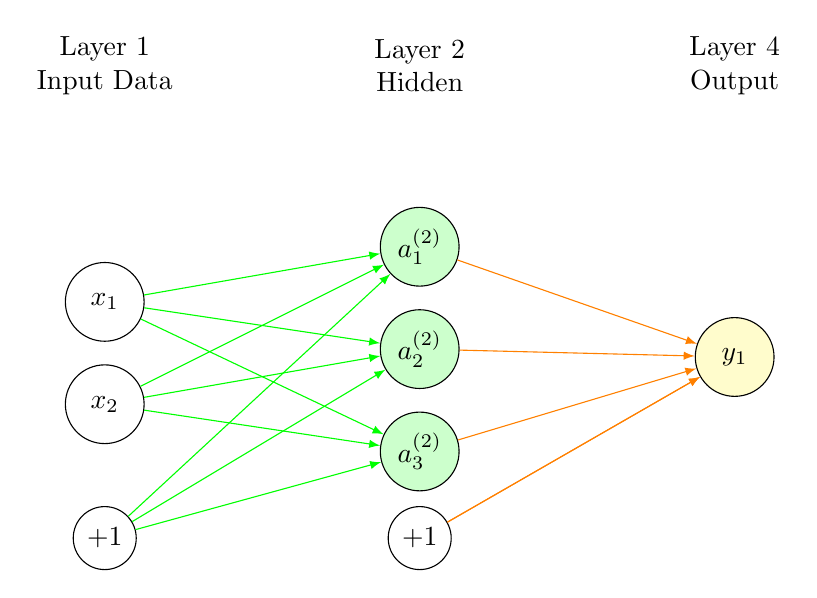
\begin{tikzpicture}[
        neuron/.style={circle, draw, minimum size=1cm, inner sep=0pt},
        bias/.style={circle, draw, minimum size=0.8cm, inner sep=0pt, fill=white},
        layer/.style={minimum width=1cm, align=center},
        connection/.style={->, >=latex}
    ]

    % Input Layer
    \foreach \i in {1,2} {
        \node[neuron] (I\i) at (1, -1.3*\i-.7) {$x_{\i}$};
    }
    \node[bias] (B1) at (1, -5) {+1};

    % Hidden Layer 1
    \foreach \i in {1,2,3} {
        \node[neuron, fill=green!20] (H1\i) at (5, -1.3*\i) {$a_{\i}^{(2)}$};
    }
    \node[bias] (B2) at (5, -5) {+1};

    % Output Layer
    \node[neuron, fill=yellow!20] (O) at (9, -2.7) {$y_{1}$};

    % Connections: Input to Hidden Layer 1
    \foreach \i in {1,2} {
        \foreach \j in {1,2,3} {
            \draw[connection, green] (I\i) -- (H1\j);
        }
    }
    \foreach \j in {1,2,3} {
        \draw[connection, green] (B1) -- (H1\j);
    }

    % Connections: Hidden Layer 2 to Output Layer
    \foreach \i in {1,2,3} {
        \draw[connection, orange] (H1\i) -- (O);
    }
    \foreach \j in {1,2} {
        \draw[connection, orange] (B2) -- (O);
    }

    % Layer Labels
    \node[layer] at (1, 1) {Layer 1 \\ Input Data};
    \node[layer] at (5, 1) {Layer 2 \\ Hidden};
    \node[layer] at (9, 1) {Layer 4 \\ Output};

    \end{tikzpicture}
    \caption{Basic NN}
    \label{fig:enter-label}
\end{figure}

The ML algorithm that this paper will explore is linear regression. So, in this paper, I will apply different gradient descent methods on ice cream sale prediction. I will predict the number of sales of ice cream bars based on the temperature outside. Let us say this is the past data of sales:

\begin{table}[h]
    \centering
    \resizebox{\textwidth}{!}{
        \begin{tabular}{ccc}
            \toprule
            \textbf{Temperature Outside (C)} & \textbf{Number of students passed by} & \textbf{Number of ice cream bars sold} \\
            \midrule
            14 & 15 & 2 \\
            18 & 27 & 5 \\
            21 & 34 & 14 \\
            30 & 38 & 16 \\
            38 & 52 & 26 \\
            \bottomrule
        \end{tabular}
    }
    \caption{Ice Cream Sales vs Temperature}
    \label{tab:ice_cream_sales}
\end{table}
The input will be two input neurons, temperature and the number of students who passed by. The output layer will be of one neuron, which is the number of ice cream bars sold. The objective is to find the best prediction of the number of ice cream bars sold.

In the neural network, the values are multiplied by the weights and a bias is added. The weights are used to add more importance to the inputs (e.g. if temperature is a more important factor when predicting the number of ice cream bars sold, the weight would be larger in value). The goal of gradient descent is to optimize the weights and bias to find the best prediction. 

The predicted output $y$ is calculated via propagating the input values through the neural network. First, each neuron in the hidden layer receives weighted input from the input layer and adds a bias term. These transformations are then passed to the output neuron which also computes a weighted sum to produce the final prediction. Mathematically, the activations of the hidden layer neurons are given by:
\[
a_{1} = x_{1}w_{11}+x_{1}w_{21}+b
\]
\[
a_{2} = x_{1}w_{12}+x_{1}w_{22}+b
\]
\[
a_{3} = x_{1}w_{13}+x_{1}w_{23}+b
\]
where $x_{1}$ and $x_{2}$ are the input values, $w_{ij}$ are the weights connecting the input neurons to the hidden neurons, and $b_i$ is the bias term. These activations are then combined in the output layer using another weighted sum:

\[y = a_{1}w_{1}+a_{2}w_{2}+a_{3}w_{3}+b\]

where $w_1$, $w_2$, and $w_3$ are the weights from the hidden layer to the output neuron, and $b$ is the bias. This process results in the final predicted value $y$.

However, no hidden layer will be implemented for our example because linear regression models do not have complex biases. So, the neural network will look like the diagram below:

\begin{figure}[h]
    \centering
    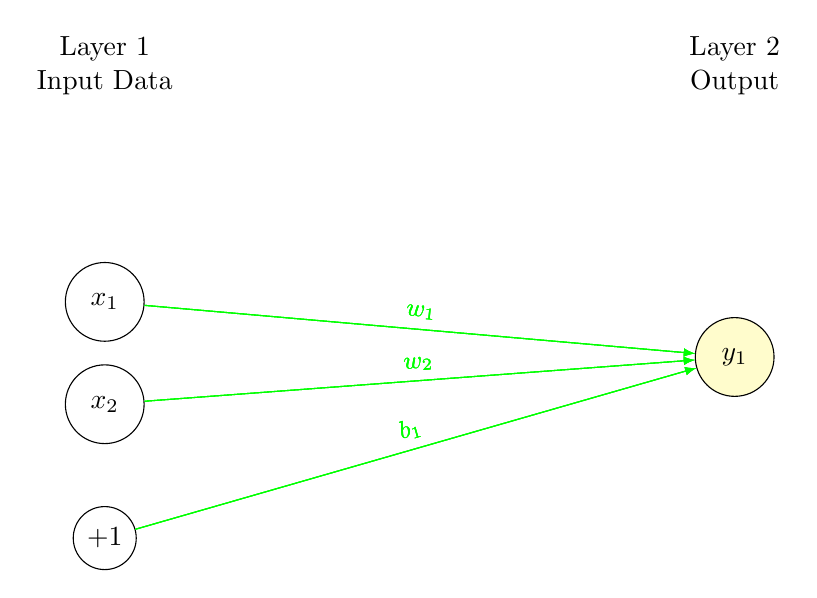
\begin{tikzpicture}[
        neuron/.style={circle, draw, minimum size=1cm, inner sep=0pt},
        bias/.style={circle, draw, minimum size=0.8cm, inner sep=0pt, fill=white},
        layer/.style={minimum width=1cm, align=center},
        connection/.style={->, >=latex}
    ]

    % Input Layer
    \foreach \i in {1,2} {
        \node[neuron] (I\i) at (1, -1.3*\i-.7) {$x_{\i}$};
    }
    \node[bias] (B1) at (1, -5) {+1};

    % Output Layer
    \node[neuron, fill=yellow!20] (O) at (9, -2.7) {$y_{1}$};

    % Connections: Input to Hidden Layer 1
    \foreach \i in {1,2} {
        \foreach \j in {1,2,3} {
            \draw[connection, green] (I\i) -- (O) node[midway, above, sloped] {\small $w_{\i}$};
        }
    }
    \foreach \j in {1,2,3} {
        \draw[connection, green] (B1) -- (O) node[midway, above, sloped] {\small $b_{1}$};
    }

    % Layer Labels
    \node[layer] at (1, 1) {Layer 1 \\ Input Data};
    \node[layer] at (9, 1) {Layer 2 \\ Output};

    \end{tikzpicture}
    \caption{NN for this paper's linear regression}
    \label{fig:enter-label}
\end{figure}

In order for a NN to train to become more accurate, the network needs to be able to know if it is incorrect. To quantify the error of the predicted output of the NN from the actual output, I can subtract the actual output value from the predicted value $y$: 

\[y_{predicted} - y_{actual}\]

This is known as the \textit{loss function}, but one problem with this loss function is that $y_{predicted}$ could be smaller than $y_{actual}$, resulting in a negative value, so typically the loss function $L(x)$ is squared, and multiplied by $\frac{1}{2}$ for easier differentiation purposes.

\[L(x) = \frac{1}{2}(y_{predicted} - y_{actual})^2\]

I will be using a dataset, so I have to calculate the average error across the entire NN. The mean squared error (MSE) is a common metric used to evaluate the performance of regression models by measuring the average squared difference between the actual and predicted values ("Mean Square Error"). The formula for the MSE is:

\[
MSE = \frac{1}{2m} \sum_{i=1}^{m} (y_{predicted} - y_{actual})^2
\]

Where \( m \) is the number of data points.

\begin{flushleft}
\textbf{Vanilla Gradient Descent}
\end{flushleft}

Gradient descent is an iterative optimization algorithm used in machine learning to improve model accuracy. It helps find the best weights and biases by minimizing the loss function $L(x)$. The smaller the loss function value, the more accurate the model is. While it is possible to find the exact minimum of $L(x)$ using calculus, that method becomes impractical for complex models. Gradient descent takes small steps in the direction that reduces the loss. The simplest form of this method is called vanilla gradient descent. To understand how it works, a basic understanding of partial derivatives is helpful:

Let $f$ be a continuous function of $n$ variables in $\mathbb{R}^n$. The partial derivative of $f$ with respect to one of its variables $x_i$, while keeping all other variables fixed, is defined as:
\[
\frac{\partial f}{\partial x_i} = \lim_{x\to 0} \frac{f(x_1,x_2, \cdots,x_i + h, x_n) - f(x_1,x_2, \cdots,x_i,\cdots,x_n)}{h} 
\]
This expression calculates the rate at which f changes as the variable xi changes, with all other variables held constant.

Example: Consider the function $f(x, y, z) = 4x^2y + 3yz^3 + z^4$. I will find the partial derivative of $f$ with respect to $z$ using the definition:
\[
\frac{\partial f}{\partial x_i} = \lim_{h\to 0} \frac{f(x,y,z+h) - f(x,y,z)}{h} 
\]
Substitute the function f(x, y, z) into the limit:
\[
\frac{\partial f}{\partial z} = \lim_{h\to 0} \frac{4x^2y + 3y(z+h)^3 + (z+h)^4 - (4x^2y + 3yz^3 + z^4)}{h} 
\]
Further simplification gives:
\[
\frac{\partial f}{\partial z} = \lim_{h\to 0} \frac{3y(3z^2h+3zh^2+h^3) +(4z^3h + 6z^2h^2 + 4zh^3 +h^4)}{h} 
\]
Factor out h from each term:
\[
\frac{\partial f}{\partial z} = \lim_{h\to 0} 9yz^2+9yzh+3yh^2 +4z^3+ 6z^2h + 4zh^2 + h^3 
\]
As h approaches 0, all terms involving h go to 0:
\[
\frac{\partial f}{\partial z} = 9yz^2+4z^3 
\]
Thus, the partial derivative of $f$ with respect to $z$ is found. Now that we understand how to compute partial derivatives, we can see how they are used in gradient descent. Imagine you are standing on a foggy hillside, trying to reach the lowest point in the terrain—the minimum of the loss function $L(x)$. You can't see the entire landscape, so instead of randomly jumping around, you take small, calculated steps downward.

The gradient ($\nabla$) is a vector of all partial derivatives of the loss function with respect to each parameter (variable). The gradient tells us the direction of steepest ascent of the function at a given point. In gradient descent, we use the gradient to determine the best direction to minimize the loss function $L(x)$, so we update each parameter $w_i$ or $b_i$ by moving in the opposite direction of its gradient (direction of steepest descent):
\[
w_{t+1} = w_t - \alpha \frac{\partial L}{\partial w_t}\text{, for }\alpha > 0
\]
\[
b_{t+1} = b_t - \alpha \frac{\partial L}{\partial b_t}\text{, for }\alpha > 0
\]
Where $\alpha$ is the learning rate, controlling step size. 

$\alpha$ is an adjustable hyperparameter, so it could be any constant, such as 0.0001. At the beginning of this process, the weights and biases are initialized with random values—just as if you started your descent from a random point on the hill. In each iteration, you "look around" by computing the gradient, then "take a step" by adjusting the weights and biases in the steepest downward direction. This process repeats until you reach the lowest possible point, where further steps no longer significantly decrease the loss. By continuously following this rule, gradient descent gradually fine-tunes the parameters to improve model accuracy.

% add more here :)
Let us start off with initial guess w1= -0.5, w2=1, b=1. The goal is to find the minimum of loss function L(x) = $12(y-y)^2$

\begin{flushleft}
\textbf{Extension: Gradient descent with Momentum}
\end{flushleft}
Similar to vanilla gradient descent, momentum gradient is nearly the same, except a new hyperparameter is introduced called momentum decay $\beta \in [0,1)$. Typical values for $\beta$ logarithmically approach 1, so some typical values might be 0.6, 0.8, 0.9, 0.99 or so, but any number between 0 and 1 is valid (``Cornell University Computational Optimization Open Textbook"). The $\beta$ controls how much of the previous update's velocity is retained when computing the current update. This allows the optimizer to accumulate velocity in a consistent direction, making convergence faster and reducing fluctuations. The update rule for gradient descent with momentum is:
\[
v = \beta v - \alpha \frac{\partial L}{\partial w_t}\text{, for }\alpha > 0
\]
\[
w_{t+1} = w_t + v
\]
If $\beta = 0$, then it is the same as vanilla gradient descent.

\begin{flushleft}
\textbf{Newton's method of Gradient Descent}
\end{flushleft}
Newton’s method has the same objective as vanilla gradient descent: to minimize the loss function $L(X)$. However, instead of searching for the minimum loss by iteratively moving in the direction of the negative gradient, Newton's method looks for the zeros of the derivative by leveraging the curvature information from the second derivative to directly estimate where the loss function reaches its minimum.

Suppose I want to find the root of a function $f(x)$, meaning I want to find $x$ such that $f(x)=0$. Newton's method starts with an initial guess $x_0$ and then refines this guess iteratively to get the x-value closest to zero. The method is based on the idea of linear approximation. At any point $x_n$, the function $f(x)$ can be approximated by its tangent line.
\[
f'(x_0)=\frac{f(x_0)}{x_0 - x_1}
\]
Solving for $x$, I get:
\[
x_1 = x_0 - \frac{f(x_0)}{f'(x_0)}
\]
$x_1$ is the x-value closer to the zero of the function. This leads to the iterative formula used in Newton's method:
\[
x_{n+1} = x_n - \frac{f(x_n)}{f'(x_n)}
\]
Newton’s method begins with an initial guess, then the iterative formula $x_{n+1} = x_n - \frac{f(x_n)}{f'(x_n)}$ is used to compute the next approximation. This is repeated until the difference between each approximation is smaller than some tolerance, meaning that the algorithm has converged.

To extend Newton's method to gradient descent, instead of finding the zeros of $f(x)$, the goal is to minimize $L(x)$ by finding the zeros of the derivative $L'(x)$. Therefore, the iterative update for Newton's method of gradient descent is given:
\[
x_{n+1} = x_n - \frac{L'(x_n)}{L''(x_n)}
\]
The second derivative, $f''(x)$, of a function provides information about the curvature of the function, meaning how its slope (rate of change) is changing at a given point. It helps us understand whether the function is concave up, concave down, or has an inflection point. If $f''(x)>0$, the function is concave up, $f''(x)<0$ is concave down, and $f''(x)=0$ is at an inflection. By dividing each step by the second derivative, the step size is adjusted dynamically. In areas of high curvature, it shrinks steps to avoid overshooting, and in flatter parts, it takes bigger steps to speed convergence.

To extend Newton's method of gradient descent to neural networks with $n$ variables, an understanding of the gradient and the Hessian matrix is crucial. The gradient, as mentioned earlier, is a vector-valued function that compiles all the partial derivatives of a multi-variable function. Similar to a derivative in single-variable calculus, a gradient represents the direction of greatest change. This also means that when the gradient of a function is set to zero, critical points can be computed, allowing a function's maximum, minimum, and saddle points to be found. The definition of a gradient follows:

Consider a function $f$: $\mathbb{R}^n \to \mathbb{R}$, where $f$ maps a vector $x = (x_1, x_2, \cdots, x_n)$ to a real number. The gradient of $f$, denoted by $\nabla f(x)$, is a vector consisting of the partial derivatives of f with respect to each variable: 
\[
\nabla f(x) = (\frac{\partial f}{\partial x_1}, \frac{\partial f}{\partial x_2}, \cdots, \frac{\partial f}{\partial x_n})
\]
Each component of the gradient vector $(\frac{\partial f}{\partial x_i}$ represents the rate of change of the function $f$ with respect to the corresponding variable $x_i$, while keeping the other variables constant. Geometrically, the gradient points in the direction of the steepest increase of the function. The magnitude of the gradient vector gives the rate of increase in that direction.

Using the example of $f(x,y,z) = 4x^2y+3yz^3 + z^4$, find $\nabla$
\[
\nabla f(x) = (\frac{\partial f}{\partial x}, \frac{\partial f}{\partial y}, \frac{\partial f}{\partial z})
\]
\[
\frac{\partial f}{\partial x}=8xy, \frac{\partial f}{\partial y} = 4x^2+3z^3, \frac{\partial f}{\partial z}=9yz^2+4z^3
\]
\[
\nabla f(x,y) = (8xy, 4x^2 + 3z^3, 9yz^2 + 4z^3)
\]
This gradient vector points radially outward from the origin and represents the direction in which the function $f(x, y, z)$ increases most rapidly. 

For multivariable functions the second derivative is a matrix of second derivatives, which is called the Hessian. In multiple variables, the first derivative is a matrix of the derivatives of the function with respect to each variable, a gradient. Similarly, the second derivative is a matrix of the derivatives of each function of the gradient with respect to each variable. This matrix is the Hessian

For a twice-differentiable scalar function $f$: $\mathbb{R}^n \to \mathbb{R}$, the Hessian matrix, denoted by $H(x)$ or simple $H$, is an $n \times n$ symmetric matrix defined as:
\[
H(x) = \begin{pmatrix}
\frac{\partial^2 f}{\partial x_1^2} & \frac{\partial^2 f}{\partial x_1 \partial x_2} & \cdots & \frac{\partial^2 f}{\partial x_1 \partial x_n} \\

\frac{\partial^2 f}{\partial x_1 \partial x_2} & \frac{\partial^2 f}{\partial x_2^2} & \cdots & \frac{\partial^2 f}{\partial x_2 \partial x_n} \\

\vdots & \vdots & \ddots & \vdots \\

\frac{\partial^2 f}{\partial x_n \partial x_1} & \frac{\partial^2 f}{\partial x_n \partial x_2} & \cdots & \frac{\partial^2 f}{\partial x_n^2}
\end{pmatrix}
\]
Each element $H_{ij} = \frac{\partial^2 f}{\partial x_i \partial x_j}$ in the Hessian matrix represents the second-order partial derivative of the function with respect to $x_i$ and $x_j$.

The Hessian is important in optimization and machine learning because it provides information about the curvature of a function. The concavity of a function can be determined using the Hessian eigenvalues.

\textbf{Definition:} (Eigenvalue and eigenvector). 
Let \( A \) be an \( n \times n \) square matrix. A scalar \( \lambda \) is called an eigenvalue of \( A \) if there exists a nonzero vector \( v \in \mathbb{R}^n \) (called an eigenvector) such that:  
\[
A v = \lambda v.
\]  
In other words, an eigenvalue \( \lambda \) represents a scalar factor by which the eigenvector \( v \) is stretched or shrunk when multiplied by \( A \). The eigenvalues of \( A \) are found by solving the characteristic equation:  
\[
\det(A - \lambda I) = 0.
\]  


\begin{theorem}
Let \( f: \mathbb{R}^n \to \mathbb{R} \) be a twice-differentiable function, and let \( H(x) \) denote its Hessian matrix at a point \( x \). The concavity or convexity of \( f \) at \( x \) is determined by the eigenvalues of \( H(x) \) as follows:  
\end{theorem}

1. \textbf{Strict Convexity (Positive Definite Hessian):}  
   If all eigenvalues of \( H(x) \) are strictly positive (\(\lambda_i > 0\) for all \( i \)), then \( H(x) \) is positive definite, and \( f(x) \) is strictly convex at \( x \).  

2. \textbf{Strict Concavity (Negative Definite Hessian):}  
   If all eigenvalues of \( H(x) \) are strictly negative (\(\lambda_i < 0\) for all \( i \)), then \( H(x) \) is negative definite, and \( f(x) \) is strictly concave at \( x \).  

3. \textbf{Saddle Point (Indefinite Hessian):}  
   If \( H(x) \) has both positive and negative eigenvalues, then \( H(x) \) is indefinite, and \( x \) is a saddle point of \( f(x) \).  

Consider an example $f(x,y) = 2x^2 + 3y^2 - xy$ function, find the function's concavity.

To find critical points, we compute the first-order derivatives:

\[
\frac{\partial f}{\partial x} = 4x - y
\]
\[
\frac{\partial f}{\partial y} = 6y - x
\]

Setting these derivatives to zero:

\[
4x - y = 0
\]
\[
6y - x = 0
\]

Solving for \( x \) and \( y \):  
From \( 4x = y \), substitute into \( 6y = x \):

\[
6(4x) = x
\]
\[
24x = x
\]
\[
x = 0, \quad y = 0
\]

Thus, the only critical point is \( (0,0) \).

Now, we compute the second-order partial derivatives:

\[
\frac{\partial^2 f}{\partial x^2} = 4, \quad \frac{\partial^2 f}{\partial y^2} = 6, \quad \frac{\partial^2 f}{\partial x \partial y} = -1
\]

Thus, the Hessian matrix is:

\[
H(x,y) =
\begin{bmatrix}
4 & -1 \\
-1 & 6
\end{bmatrix}
\]

Evaluating at \( (0,0) \):

\[
H(0,0) =
\begin{bmatrix}
4 & -1 \\
-1 & 6
\end{bmatrix}
\]

To determine the nature of the critical point, we find the eigenvalues of \( H(0,0) \) by solving:
\[
\det \left( H(0,0) - \lambda I \right) = 0
\]
\[
\det \begin{bmatrix} 4 - \lambda & -1 \\ -1 & 6 - \lambda \end{bmatrix} = 0
\]
Expanding the determinant:
\[
(4 - \lambda)(6 - \lambda) - (-1)(-1) = 0
\]
\[
(4 - \lambda)(6 - \lambda) - 1 = 0
\]
\[
\lambda^2 - 10\lambda + 23 = 0
\]
Solving for \( \lambda \):
\[
\lambda = \frac{10 \pm \sqrt{100 - 92}}{2} = \frac{10 \pm \sqrt{8}}{2} = \frac{10 \pm 2\sqrt{2}}{2} = 5 \pm \sqrt{2}
\]

Since both eigenvalues are positive, \( H(0,0) \) is positive definite, that is, \( f(x,y) \) has a local minimum at (0,0).

Now that we understand the Hessian and the gradient, we can generalize Newton's multi-variable optimization method. Recalling Newton's method for a single-variable function \( f(x) \), the iterative update rule is given by:
\[
x_{n+1} = x_n - \frac{f(x_n)}{f'(x_n)}
\]

We can now extend this method to functions of multiple variables. Suppose that we have a function \( f: \mathbb{R}^n \to \mathbb{R} \) that we want to minimize. Instead of using the derivative \( f'(x) \), we now use the gradient \( \nabla f(x) \), and instead of the second derivative \( f''(x) \), we use the Hessian matrix \( H(x) \), which consists of second-order partial derivatives.

Newton's update in multiple dimensions is then:

\[
\mathbf{x}_{n+1} = \mathbf{x}_n - H(\mathbf{x}_n)^{-1} \nabla f(\mathbf{x}_n)
\]

where \( \mathbf{x}_n \) is the current iterate (a vector in \( \mathbb{R}^n \)),
\( \nabla f(\mathbf{x}) \) is the gradient vector \( \left( \frac{\partial f}{\partial x_1}, \frac{\partial f}{\partial x_2}, \dots, \frac{\partial f}{\partial x_n} \right) \), and \( H(\mathbf{x}) \) is the Hessian matrix.

In optimization problems, especially in machine learning algorithms like Newton's method, the Hessian matrix is used to refine the search for a minimum. Newton's method, which updates the parameters of a function based on both the gradient and the Hessian, utilizes the curvature information to adjust the step size, potentially leading to faster convergence compared to methods that only use the gradient, like Vanilla Gradient Descent. However, calculating the Hessian can be computationally expensive, especially for functions with a large number of variables, which is why it is often approximated or used selectively in practice.

\begin{flushleft}
\textbf{Application of Vanilla and Newton's Method of Gradient Descent}
\end{flushleft}
Now that I've established the mathematical basis of both Vanilla and Newton's methods of gradient descent, I will now compare and apply them to a practical scenario. Using the data table introduced earlier, I will train a small neural network to predict ice cream sales based on temperature and the number of students who passed.

To illustrate the training process, I will manually compute the initial iterations of both methods, demonstrating their step-by-step calculations of the neural network training. However, given the computational complexity and repetitiveness of the full training process, I will implement the remaining iterations in Python. The primary metric for comparison will be the convergence rates, measured by the number of iterations. Finally, I will present a broader analysis of their performance in the conclusion.


There are a variety of criterion for determining convergence, such as setting a maximum number of iterations for neural network training, but because I need to compare the convergence of both methods via iterations, convergence of the neural network training will be defined as occurring when the step size of the gradient becomes smaller than a chosen tolerance level, specifically:  

\[
|x_{n+1} - x_n| < 10^{-3}
\]

Once this condition is met, the method is considered to have converged.  

Now that I've established the criteria for convergence, I will manually compute the initial iterations of Vanilla gradient descent.


I introduce an intercept term \( x_0 = 1 \) to account for the bias term, so our feature matrix \( X \) is:
\[
X =
\begin{bmatrix}
1 & 14 & 15 \\
1 & 18 & 27 \\
1 & 21 & 34 \\
1 & 30 & 38 \\
1 & 38 & 52
\end{bmatrix}
\]
Let \( \theta = [\theta_0, \theta_1, \theta_2] \) be our parameter vector, initialized randomly.

Step 1: Compute Predictions
\[
y_{predicted}(X) = \theta_0 + \theta_1 x_1 + \theta_2 x_2
\]
Assume the initial values:  
\[
\theta_0 = 0.1, \quad \theta_1 = 0.2, \quad \theta_2 = 0.3
\]
Compute predictions:
\[
\begin{aligned}
y_{predicted}(x_1) &= 0.1 + (0.2)(14) + (0.3)(15) = 0.1 + 2.8 + 4.5 = 7.4 \\
y_{predicted}(x_2) &= 0.1 + (0.2)(18) + (0.3)(27) = 0.1 + 3.6 + 8.1 = 11.8 \\
y_{predicted}(x_3) &= 0.1 + (0.2)(21) + (0.3)(34) = 0.1 + 4.2 + 10.2 = 14.5 \\
y_{predicted}(x_4) &= 0.1 + (0.2)(30) + (0.3)(38) = 0.1 + 6.0 + 11.4 = 17.5 \\
y_{predicted}(x_5) &= 0.1 + (0.2)(38) + (0.3)(52) = 0.1 + 7.6 + 15.6 = 23.3
\end{aligned}
\]

Step 2: Compute Error
\[
\text{error} = y_{predicted} - y_{actual}\]

\[
\begin{aligned}
e_1 &= 7.4 - 2 = 5.4 \\
e_2 &= 11.8 - 5 = 6.8 \\
e_3 &= 14.5 - 14 = 0.5 \\
e_4 &= 17.5 - 16 = 1.5 \\
e_5 &= 23.3 - 26 = -2.7
\end{aligned}
\]
Step 3: Compute Partial Derivatives (Gradient)
\[
\frac{\partial J}{\partial \theta_k} = \frac{1}{m} \sum_{i=1}^{m} e_i x_{ik}
\]
Gradient for \( \theta_0 \):
\[
\frac{\partial J}{\partial \theta_0} = \frac{1}{5} (5.4 + 6.8 + 0.5 + 1.5 - 2.7) = \frac{11.5}{5} = 2.3
\]
Gradient for \( \theta_1 \):
\[
\frac{\partial J}{\partial \theta_1} = \frac{1}{5} (5.4(14) + 6.8(18) + 0.5(21) + 1.5(30) - 2.7(38))
\]
\[
= \frac{1}{5} (75.6 + 122.4 + 10.5 + 45 - 102.6) = \frac{150.9}{5} = 30.18
\]
Gradient for \( \theta_2 \):
\[
\frac{\partial J}{\partial \theta_2} = \frac{1}{5} (5.4(15) + 6.8(27) + 0.5(34) + 1.5(38) - 2.7(52))
\]
\[
= \frac{1}{5} (81 + 183.6 + 17 + 57 - 140.4) = \frac{198.2}{5} = 39.64
\]

Now that I've calculated the partial derivatives of the loss function, I can now update the parameters using the gradient descent formula:
\[
\theta_k = \theta_k - \alpha \frac{\partial J}{\partial \theta_k}
\]
For \( \alpha = 0.01 \):
\[
\begin{aligned}
\theta_0 &= 0.1 - (0.01)(2.3) = 0.077 \\
\theta_1 &= 0.2 - (0.01)(30.18) = -0.1018 \\
\theta_2 &= 0.3 - (0.01)(39.64) = -0.0964
\end{aligned}
\]

\[
\vdots
\]

These calculations are iterated until convergence is reached. The rest of the calculations were done in Python (Appendix A). However, the alpha value was reduced to 0.001, and the initial theta values is randomly assigned between the values of 0 to 1, set with a random seed of 42.

\begin{figure}[h]
    \centering
    \includegraphics[width=0.75\linewidth]{graphGrad.png}
    \caption{Loss Curve for Vanilla Gradient Descent}
    \label{fig:enter-label}
\end{figure}

Newton's method has the same beginning calculations as Vanilla, but in addition to the gradient being calculated, the Hessian is also calculated.

Step 1: Compute Predictions
\[
\hat{y} = X \cdot \theta
\]

Using some random initial values of \( \theta \), say:

\[
\theta = \begin{bmatrix} 0.1 \\ 0.2 \\ 0.3 \end{bmatrix}
\]

We calculate predictions using matrix multiplication:
\[
y_{predicted} = \begin{bmatrix}
1 & 14 & 15 \\
1 & 18 & 27 \\
1 & 21 & 34 \\
1 & 30 & 38 \\
1 & 38 & 52
\end{bmatrix}
\cdot
\begin{bmatrix} 0.1 \\ 0.2 \\ 0.3 \end{bmatrix}
\]
\[
y_{predicted} =
\begin{bmatrix}
0.1 + (14 \times 0.2) + (15 \times 0.3) \\
0.1 + (18 \times 0.2) + (27 \times 0.3) \\
0.1 + (21 \times 0.2) + (34 \times 0.3) \\
0.1 + (30 \times 0.2) + (38 \times 0.3) \\
0.1 + (38 \times 0.2) + (52 \times 0.3)
\end{bmatrix}
\]
Resulting in:
\[
y_{predicted} = \begin{bmatrix} 7.4 \\ 11.8 \\ 14.5 \\ 17.5 \\ 23.3 \end{bmatrix}
\]
Step 2: Compute Error
The error is determined by subtracting the actual values from the predicted values:
\[
\text{Error} = y_{predicted} - y_{actual}
\]
\[
\begin{bmatrix} 7.4 \\ 11.8 \\ 14.5 \\ 17.5 \\ 23.3 \end{bmatrix} - \begin{bmatrix} 2 \\ 5 \\ 14 \\ 16 \\ 26 \end{bmatrix}
=
\begin{bmatrix} 5.4 \\ 6.8 \\ 0.5 \\ 1.5 \\ -2.7 \end{bmatrix}
\]
Step 3: Compute Gradient
\[
\nabla J = \frac{1}{m} X^T (\hat{y} - y)
\]
Computing \( X^T \):
\[
X^T =
\begin{bmatrix}
1 & 1 & 1 & 1 & 1 \\
14 & 18 & 21 & 30 & 38 \\
15 & 27 & 34 & 38 & 52
\end{bmatrix}
\]

\[
X^T (\hat{y} - y) =
\begin{bmatrix}
1 & 1 & 1 & 1 & 1 \\
14 & 18 & 21 & 30 & 38 \\
15 & 27 & 34 & 38 & 52
\end{bmatrix}
\cdot
\begin{bmatrix} 5.4 \\ 6.8 \\ 0.5 \\ 1.5 \\ -2.7 \end{bmatrix}
\]

\[
=
\begin{bmatrix}
11.5 \\
150.9 \\
198.2
\end{bmatrix}
\]

\[
\nabla J = \frac{1}{5} \begin{bmatrix} 11.5 \\150.9 \\198.2 \end{bmatrix} =
\begin{bmatrix} 2.3 \\ 30.18 \\ 39.64 \end{bmatrix}
\]

Step 4: Compute the Hessian Matrix

The Hessian is:
\[
H = \frac{1}{m} \sum_{i=1}^{m} x_{ij} x_{ik}
\]
\[
H =
\begin{bmatrix}
1 & 14 & 15 \\
1 & 18 & 27 \\
1 & 21 & 34 \\
1 & 30 & 38 \\
1 & 38 & 52
\end{bmatrix}^T
\begin{bmatrix}
1 & 14 & 15 \\
1 & 18 & 27 \\
1 & 21 & 34 \\
1 & 30 & 38 \\
1 & 38 & 52
\end{bmatrix}
\]
Computing Hessian \( H \):
\[
H =
\frac{1}{5}
\begin{bmatrix}
5 & 121 & 166 \\
121 & 3305 & 4526 \\
166 & 4526 & 6258
\end{bmatrix}
\]
\[
H =
\begin{bmatrix}
1 & \frac{121}{5} & \frac{166}{5} \\
\frac{121}{5} & 661 & \frac{4526}/5 \\
\frac{166}{5} & \frac{4526}{5} & \frac{6258}{5}
\end{bmatrix}
\]
\[
H^{-1} \approx
\begin{bmatrix}
8.79 & -0.26 & -0.04 \\
-0.26 & 0.17 & 0.11 \\
-0.044 & -0.11 & 0.084
\end{bmatrix}
\]

Step 5: Compute Parameter Update
\[
\theta_{\text{new}} = \theta - \alpha H^{-1} \cdot \nabla J
\]

\[
\theta_{\text{new}} =
\begin{bmatrix} 0.1 \\ 0.2 \\ 0.3 \end{bmatrix} - \alpha
\begin{bmatrix}
8.79 & -0.26 & -0.04 \\
-0.26 & 0.17 & 0.11 \\
-0.044 & -0.11 & 0.084
\end{bmatrix}
\cdot
\begin{bmatrix} 2.3 \\ 30.18 \\ 39.64 \end{bmatrix}
\]

Solving, given alpha is $0.01$:
\[
\theta_{\text{new}} = \begin{bmatrix} -0.007846\\ 0.11107\\ 0.300912 \end{bmatrix}
\]

This process repeats until convergence.

The rest of the calculations were also done in Python (Appendix A). Unlike Vanilla Gradient Descent, Newton’s method typically converges in fewer steps due to its use of the Hessian, but it comes at the cost of higher computational complexity. The alpha value was 0.01 unlike Vanilla, but the initial theta values for both methods are the same.

\begin{figure}[h]
    \centering
    \includegraphics[width=0.75\linewidth]{graphNewtons.png}
    \caption{Loss Curve for Newton's Method of Gradient Descent}
    \label{fig:enter-label}
\end{figure}

\begin{flushleft}
\textbf{Comparison of Vanilla and Newton's Method of Gradient Descent}
\end{flushleft}

After running both Vanilla and Newton's methods through the Python program, the loss score for the 1st, 100th, 500th, and final iteration (or ``epoch") was recorded. Each value was rounded to the third decimal place for consistency. 
\begin{table}[h]
    \centering
    \begin{tabular}{|c|c|c|}
        \hline
        & \textbf{Vanilla} & \textbf{Newton} \\ \hline
        \textbf{Loss (1st epoch)} & 108.545 & 128.301 \\ \hline
        \textbf{Loss (100th epoch)} & 1.645 & 17.422 \\ \hline
        \textbf{Loss (500th epoch)} & 1.461 & 0.274 \\ \hline
        \textbf{Last loss} & 1.154 & 0.268 \\ \hline
    \end{tabular}
    \caption{Comparison of Vanilla and Newton's gradient descent results}
    \label{tab:optimization_comparison}
\end{table}

As seen in Table \ref{tab:optimization_comparison}, Newton’s method initially exhibited a higher loss than Vanilla gradient descent in the first epoch. However, as training progressed, Newton’s method significantly outperformed Vanilla in terms of convergence speed and final loss value. By the 500th epoch, Newton’s method had already reduced the loss to 0.274, whereas Vanilla gradient descent was still at 1.461. This trend continued, with Newton ultimately converging to a final loss of 0.268, compared to Vanilla’s 1.154.

\begin{figure}[h]
    \centering
    \includegraphics[width=0.75\linewidth]{graphCompare.png}
    \caption{Loss curves of both functions}
    \label{fig:enter-label}
\end{figure}

The graph further illustrates the differences in convergence behavior. Newton’s method reached its optimal loss at epoch 904, nearly twice as fast as Vanilla gradient descent, which required 1,826 epochs to converge. This efficiency is due to Newton’s method utilizing second-order derivatives, allowing for more informed step size adjustments and faster movement toward the minimum.

Overall, the results demonstrate that while Newton’s method may start with a higher initial loss, it converges significantly faster and to a lower loss value compared to Vanilla gradient descent. Additional data supporting these findings can be found in Appendix B.

\break
\begin{flushleft}
\textbf{Conclusion}
\end{flushleft}

The exploration of different gradient descent methods—Vanilla and Newton’s—provided valuable insights into their convergence behaviors and computational trade-offs when training a linear regression model. This study aimed to analyze how these two optimization techniques impact the number of iterations required for convergence, ultimately affecting the efficiency of machine learning model training. Through both manual calculations and computational simulations using Python, a clear distinction between the two methods emerged.

Vanilla gradient descent, the most basic form of the algorithm, follows a steady, uniform step size dictated by the learning rate $\alpha$. It does not take into account the curvature of the function, making its updates relatively slow and requiring a significantly larger number of iterations to reach convergence. In contrast, Newton’s method incorporates second-order derivative information through the Hessian matrix, dynamically adjusting step sizes based on the curvature of the loss function. This approach enables faster convergence by taking more efficient steps toward the minimum, albeit at the cost of increased computational complexity.

The experimental results confirmed these theoretical expectations. Initially, Newton’s method exhibited a higher loss than Vanilla gradient descent. However, as training progressed, Newton’s method demonstrated superior convergence speed, ultimately achieving a lower loss value in fewer iterations. Specifically, while Vanilla gradient descent required 1,826 epochs to reach convergence, Newton’s method achieved it nearly twice as fast, converging at epoch 904. Furthermore, the final loss of Newton’s method (0.268) was significantly lower than that of Vanilla gradient descent (1.154), highlighting its improved accuracy in finding the optimal parameter values.

Despite its advantages in convergence speed, Newton’s method presents challenges that limit its widespread application, particularly in large-scale machine learning problems. The need to compute the Hessian matrix and its inverse at each iteration imposes a heavy computational burden, making the method impractical for high-dimensional datasets. On the other hand, Vanilla gradient descent, while slower, remains computationally efficient and widely used in deep learning applications where computing second-order derivatives is infeasible. 

These findings emphasize the importance of selecting the appropriate optimization technique based on the specific requirements of a given problem. For small-scale models or scenarios where computational resources are not a constraint, Newton’s method can be an excellent choice due to its rapid convergence. However, in real-world applications with high-dimensional data, Vanilla gradient descent (or its more advanced variants such as Momentum or Adam) remains a more viable solution due to its simplicity and scalability.

This study provides a foundational understanding of optimization techniques in machine learning, particularly in the context of linear regression models. Future research could expand upon this work by exploring additional gradient descent variants, such as stochastic and mini-batch gradient descent, to assess their performance across different problem domains. Additionally, applying these methods to more complex neural network architectures could provide further insights into their practical utility in modern AI applications.

In conclusion, the choice of optimization algorithm plays a crucial role in determining the efficiency and accuracy of machine learning models. While Newton’s method excels in rapid convergence, its computational demands make it less practical for large-scale problems. Vanilla gradient descent, though slower, remains a fundamental and widely used technique due to its adaptability and ease of implementation. As machine learning continues to evolve, ongoing advancements in optimization methods will further enhance the training efficiency of AI models, shaping the future of artificial intelligence and its applications.

% iterations example
% Put the works-cited on a separate page.
\newpage
\appendix

\begin{center}
    {\Huge \textbf{Appendix}}
\end{center}

\section{Python Implementation Details}
\label{sec:appendixA}
The Python implementation used the NumPy libraries. The neural network was implemented as follows.

\begin{lstlisting}
import numpy as np

temperature = np.array([14, 18, 21, 30, 38])
num_students = np.array([15, 27, 34, 38, 52])

# Array of amount of ice cream sold; price from temperature and students
sold = np.array([2, 5, 14, 16, 26])

# Stack features together
X = np.column_stack((temperature, num_students))
y = sold

np.random.seed(42)
theta = np.random.rand(X.shape[1] + 1) # Parameters for each feature and the intercept
alphaGrad = 0.001  # Learning rate for vanilla descent
alphaNewton = 0.01  # Learning rate for newton's descent
iterations = 10000  # Number of iterations

def compute_cost(X, y, theta):
    m = len(y)
    predictions = X.dot(theta)

    cost = (1/m) * np.mean((predictions - y) ** 2) / 2
    return cost

def gradient_descent(X, y, theta, alpha, num_iters, tolerance=1e-3):
    m = len(y) 
    n = len(theta)
    J_history = []

    for i in range(num_iters):
        predictions = []
        for j in range(m):
            prediction = 0
            for k in range(n):
                prediction += theta[k] * X[j][k]
            predictions.append(prediction)

        errors = [predictions[j] - y[j] for j in range(m)]

        derivative = [0] * n
        for k in range(n):
            sum_errors = 0
            for j in range(m):
              sum_errors += errors[j]*X[j][k]
            derivative[k] = (1 / m) * sum_errors

        step_size = 0
        for k in range(n):
            step = alpha * derivative[k]
            theta[k] -= step
            step_size += step**2

        step_size_norm = step_size**0.5

        if step_size_norm < tolerance:
          print(f"Stopping early at iteration {i}")
          break

        cost = compute_cost(X, y, theta)
        if (i == 1 or i %100 == 0):
          print(f"cost: {cost}, iteration: {i}")
        J_history.append(cost)

    return theta, J_history

def newton_descent(X, y, theta, alpha, num_iters, tolerance=1e-3):
    m = len(y)  
    n = len(theta) 
    J_history = []

    for i in range(num_iters):
        predictions = []
        for j in range(m):
            prediction = sum(theta[k] * X[j][k] for k in range(n))
            predictions.append(prediction)

        errors = [predictions[j] - y[j] for j in range(m)]

        gradient = [0] * n
        for k in range(n):
            sum_errors = sum(errors[j] * X[j][k] for j in range(m))
            gradient[k] = (1 / m) * sum_errors

        hessian = [[0] * n for _ in range(n)]
        for k1 in range(n):
            for k2 in range(n):
                sum_second_derivatives = sum(X[j][k1] * X[j][k2] for j in range(m))
                hessian[k1][k2] = (1 / m) * sum_second_derivatives

        hessian_inv = np.linalg.inv(hessian)  # Inverting Hessian
        step_direction = np.dot(hessian_inv, gradient)

        for k in range(n):
            theta[k] -= alpha * step_direction[k]

        step_size_squared = sum(step_direction[k] ** 2 for k in range(n))
        step_size = step_size_squared ** 0.5

        # Compute cost for tracking
        cost = compute_cost(X, y, theta)
        if (i%100 == 0 or i == 1):
          print(f"Iteration {i}, Cost: {cost}")   

        if step_size < tolerance:
            print(f"Stopping early at iteration {i}, Step size: {step_size:.6f}, cost: {cost}")
            break
          
        J_history.append(cost)

    return theta, J_history

X_bias = np.hstack([np.ones((X.shape[0], 1)), X])

# Run Vanilla gradient descent
print("Vanilla:")
final_theta, J_history = gradient_descent(X_bias, y, theta, alphaGrad, iterations)
# Run Newton's method of gradient descent
print("Newton's:")
final_theta2, J_history2 = newton_descent(X_bias, y, theta, alphaNewton, iterations)
\end{lstlisting}
\newpage
\section{Additional Data of Loss Values}
\label{sec:appendixB}
This section provides additional data collected from running both Vanilla and Newton's gradient descent methods. The loss values were recorded at regular intervals to observe the convergence trends. First, Vanilla is listed, then Newton's method loss follows.

\begin{figure}[h]
    \centering
    \includegraphics[width=0.75\linewidth]{image.png}
\end{figure}

% \bibliographystyle{mla13.sty}
% \bibliography{references}


\end{document}
